% Options for packages loaded elsewhere
\PassOptionsToPackage{unicode}{hyperref}
\PassOptionsToPackage{hyphens}{url}
\PassOptionsToPackage{dvipsnames,svgnames,x11names}{xcolor}
%
\documentclass[
  letterpaper,
  DIV=11,
  numbers=noendperiod]{scrartcl}

\usepackage{amsmath,amssymb}
\usepackage{iftex}
\ifPDFTeX
  \usepackage[T1]{fontenc}
  \usepackage[utf8]{inputenc}
  \usepackage{textcomp} % provide euro and other symbols
\else % if luatex or xetex
  \usepackage{unicode-math}
  \defaultfontfeatures{Scale=MatchLowercase}
  \defaultfontfeatures[\rmfamily]{Ligatures=TeX,Scale=1}
\fi
\usepackage{lmodern}
\ifPDFTeX\else  
    % xetex/luatex font selection
\fi
% Use upquote if available, for straight quotes in verbatim environments
\IfFileExists{upquote.sty}{\usepackage{upquote}}{}
\IfFileExists{microtype.sty}{% use microtype if available
  \usepackage[]{microtype}
  \UseMicrotypeSet[protrusion]{basicmath} % disable protrusion for tt fonts
}{}
\makeatletter
\@ifundefined{KOMAClassName}{% if non-KOMA class
  \IfFileExists{parskip.sty}{%
    \usepackage{parskip}
  }{% else
    \setlength{\parindent}{0pt}
    \setlength{\parskip}{6pt plus 2pt minus 1pt}}
}{% if KOMA class
  \KOMAoptions{parskip=half}}
\makeatother
\usepackage{xcolor}
\setlength{\emergencystretch}{3em} % prevent overfull lines
\setcounter{secnumdepth}{-\maxdimen} % remove section numbering
% Make \paragraph and \subparagraph free-standing
\makeatletter
\ifx\paragraph\undefined\else
  \let\oldparagraph\paragraph
  \renewcommand{\paragraph}{
    \@ifstar
      \xxxParagraphStar
      \xxxParagraphNoStar
  }
  \newcommand{\xxxParagraphStar}[1]{\oldparagraph*{#1}\mbox{}}
  \newcommand{\xxxParagraphNoStar}[1]{\oldparagraph{#1}\mbox{}}
\fi
\ifx\subparagraph\undefined\else
  \let\oldsubparagraph\subparagraph
  \renewcommand{\subparagraph}{
    \@ifstar
      \xxxSubParagraphStar
      \xxxSubParagraphNoStar
  }
  \newcommand{\xxxSubParagraphStar}[1]{\oldsubparagraph*{#1}\mbox{}}
  \newcommand{\xxxSubParagraphNoStar}[1]{\oldsubparagraph{#1}\mbox{}}
\fi
\makeatother

\usepackage{color}
\usepackage{fancyvrb}
\newcommand{\VerbBar}{|}
\newcommand{\VERB}{\Verb[commandchars=\\\{\}]}
\DefineVerbatimEnvironment{Highlighting}{Verbatim}{commandchars=\\\{\}}
% Add ',fontsize=\small' for more characters per line
\usepackage{framed}
\definecolor{shadecolor}{RGB}{241,243,245}
\newenvironment{Shaded}{\begin{snugshade}}{\end{snugshade}}
\newcommand{\AlertTok}[1]{\textcolor[rgb]{0.68,0.00,0.00}{#1}}
\newcommand{\AnnotationTok}[1]{\textcolor[rgb]{0.37,0.37,0.37}{#1}}
\newcommand{\AttributeTok}[1]{\textcolor[rgb]{0.40,0.45,0.13}{#1}}
\newcommand{\BaseNTok}[1]{\textcolor[rgb]{0.68,0.00,0.00}{#1}}
\newcommand{\BuiltInTok}[1]{\textcolor[rgb]{0.00,0.23,0.31}{#1}}
\newcommand{\CharTok}[1]{\textcolor[rgb]{0.13,0.47,0.30}{#1}}
\newcommand{\CommentTok}[1]{\textcolor[rgb]{0.37,0.37,0.37}{#1}}
\newcommand{\CommentVarTok}[1]{\textcolor[rgb]{0.37,0.37,0.37}{\textit{#1}}}
\newcommand{\ConstantTok}[1]{\textcolor[rgb]{0.56,0.35,0.01}{#1}}
\newcommand{\ControlFlowTok}[1]{\textcolor[rgb]{0.00,0.23,0.31}{\textbf{#1}}}
\newcommand{\DataTypeTok}[1]{\textcolor[rgb]{0.68,0.00,0.00}{#1}}
\newcommand{\DecValTok}[1]{\textcolor[rgb]{0.68,0.00,0.00}{#1}}
\newcommand{\DocumentationTok}[1]{\textcolor[rgb]{0.37,0.37,0.37}{\textit{#1}}}
\newcommand{\ErrorTok}[1]{\textcolor[rgb]{0.68,0.00,0.00}{#1}}
\newcommand{\ExtensionTok}[1]{\textcolor[rgb]{0.00,0.23,0.31}{#1}}
\newcommand{\FloatTok}[1]{\textcolor[rgb]{0.68,0.00,0.00}{#1}}
\newcommand{\FunctionTok}[1]{\textcolor[rgb]{0.28,0.35,0.67}{#1}}
\newcommand{\ImportTok}[1]{\textcolor[rgb]{0.00,0.46,0.62}{#1}}
\newcommand{\InformationTok}[1]{\textcolor[rgb]{0.37,0.37,0.37}{#1}}
\newcommand{\KeywordTok}[1]{\textcolor[rgb]{0.00,0.23,0.31}{\textbf{#1}}}
\newcommand{\NormalTok}[1]{\textcolor[rgb]{0.00,0.23,0.31}{#1}}
\newcommand{\OperatorTok}[1]{\textcolor[rgb]{0.37,0.37,0.37}{#1}}
\newcommand{\OtherTok}[1]{\textcolor[rgb]{0.00,0.23,0.31}{#1}}
\newcommand{\PreprocessorTok}[1]{\textcolor[rgb]{0.68,0.00,0.00}{#1}}
\newcommand{\RegionMarkerTok}[1]{\textcolor[rgb]{0.00,0.23,0.31}{#1}}
\newcommand{\SpecialCharTok}[1]{\textcolor[rgb]{0.37,0.37,0.37}{#1}}
\newcommand{\SpecialStringTok}[1]{\textcolor[rgb]{0.13,0.47,0.30}{#1}}
\newcommand{\StringTok}[1]{\textcolor[rgb]{0.13,0.47,0.30}{#1}}
\newcommand{\VariableTok}[1]{\textcolor[rgb]{0.07,0.07,0.07}{#1}}
\newcommand{\VerbatimStringTok}[1]{\textcolor[rgb]{0.13,0.47,0.30}{#1}}
\newcommand{\WarningTok}[1]{\textcolor[rgb]{0.37,0.37,0.37}{\textit{#1}}}

\providecommand{\tightlist}{%
  \setlength{\itemsep}{0pt}\setlength{\parskip}{0pt}}\usepackage{longtable,booktabs,array}
\usepackage{calc} % for calculating minipage widths
% Correct order of tables after \paragraph or \subparagraph
\usepackage{etoolbox}
\makeatletter
\patchcmd\longtable{\par}{\if@noskipsec\mbox{}\fi\par}{}{}
\makeatother
% Allow footnotes in longtable head/foot
\IfFileExists{footnotehyper.sty}{\usepackage{footnotehyper}}{\usepackage{footnote}}
\makesavenoteenv{longtable}
\usepackage{graphicx}
\makeatletter
\def\maxwidth{\ifdim\Gin@nat@width>\linewidth\linewidth\else\Gin@nat@width\fi}
\def\maxheight{\ifdim\Gin@nat@height>\textheight\textheight\else\Gin@nat@height\fi}
\makeatother
% Scale images if necessary, so that they will not overflow the page
% margins by default, and it is still possible to overwrite the defaults
% using explicit options in \includegraphics[width, height, ...]{}
\setkeys{Gin}{width=\maxwidth,height=\maxheight,keepaspectratio}
% Set default figure placement to htbp
\makeatletter
\def\fps@figure{htbp}
\makeatother
% definitions for citeproc citations
\NewDocumentCommand\citeproctext{}{}
\NewDocumentCommand\citeproc{mm}{%
  \begingroup\def\citeproctext{#2}\cite{#1}\endgroup}
\makeatletter
 % allow citations to break across lines
 \let\@cite@ofmt\@firstofone
 % avoid brackets around text for \cite:
 \def\@biblabel#1{}
 \def\@cite#1#2{{#1\if@tempswa , #2\fi}}
\makeatother
\newlength{\cslhangindent}
\setlength{\cslhangindent}{1.5em}
\newlength{\csllabelwidth}
\setlength{\csllabelwidth}{3em}
\newenvironment{CSLReferences}[2] % #1 hanging-indent, #2 entry-spacing
 {\begin{list}{}{%
  \setlength{\itemindent}{0pt}
  \setlength{\leftmargin}{0pt}
  \setlength{\parsep}{0pt}
  % turn on hanging indent if param 1 is 1
  \ifodd #1
   \setlength{\leftmargin}{\cslhangindent}
   \setlength{\itemindent}{-1\cslhangindent}
  \fi
  % set entry spacing
  \setlength{\itemsep}{#2\baselineskip}}}
 {\end{list}}
\usepackage{calc}
\newcommand{\CSLBlock}[1]{\hfill\break\parbox[t]{\linewidth}{\strut\ignorespaces#1\strut}}
\newcommand{\CSLLeftMargin}[1]{\parbox[t]{\csllabelwidth}{\strut#1\strut}}
\newcommand{\CSLRightInline}[1]{\parbox[t]{\linewidth - \csllabelwidth}{\strut#1\strut}}
\newcommand{\CSLIndent}[1]{\hspace{\cslhangindent}#1}

\KOMAoption{captions}{tableheading}
\makeatletter
\@ifpackageloaded{tcolorbox}{}{\usepackage[skins,breakable]{tcolorbox}}
\@ifpackageloaded{fontawesome5}{}{\usepackage{fontawesome5}}
\definecolor{quarto-callout-color}{HTML}{909090}
\definecolor{quarto-callout-note-color}{HTML}{0758E5}
\definecolor{quarto-callout-important-color}{HTML}{CC1914}
\definecolor{quarto-callout-warning-color}{HTML}{EB9113}
\definecolor{quarto-callout-tip-color}{HTML}{00A047}
\definecolor{quarto-callout-caution-color}{HTML}{FC5300}
\definecolor{quarto-callout-color-frame}{HTML}{acacac}
\definecolor{quarto-callout-note-color-frame}{HTML}{4582ec}
\definecolor{quarto-callout-important-color-frame}{HTML}{d9534f}
\definecolor{quarto-callout-warning-color-frame}{HTML}{f0ad4e}
\definecolor{quarto-callout-tip-color-frame}{HTML}{02b875}
\definecolor{quarto-callout-caution-color-frame}{HTML}{fd7e14}
\makeatother
\makeatletter
\@ifpackageloaded{caption}{}{\usepackage{caption}}
\AtBeginDocument{%
\ifdefined\contentsname
  \renewcommand*\contentsname{Table of contents}
\else
  \newcommand\contentsname{Table of contents}
\fi
\ifdefined\listfigurename
  \renewcommand*\listfigurename{List of Figures}
\else
  \newcommand\listfigurename{List of Figures}
\fi
\ifdefined\listtablename
  \renewcommand*\listtablename{List of Tables}
\else
  \newcommand\listtablename{List of Tables}
\fi
\ifdefined\figurename
  \renewcommand*\figurename{Figure}
\else
  \newcommand\figurename{Figure}
\fi
\ifdefined\tablename
  \renewcommand*\tablename{Table}
\else
  \newcommand\tablename{Table}
\fi
}
\@ifpackageloaded{float}{}{\usepackage{float}}
\floatstyle{ruled}
\@ifundefined{c@chapter}{\newfloat{codelisting}{h}{lop}}{\newfloat{codelisting}{h}{lop}[chapter]}
\floatname{codelisting}{Listing}
\newcommand*\listoflistings{\listof{codelisting}{List of Listings}}
\makeatother
\makeatletter
\makeatother
\makeatletter
\@ifpackageloaded{caption}{}{\usepackage{caption}}
\@ifpackageloaded{subcaption}{}{\usepackage{subcaption}}
\makeatother

\ifLuaTeX
  \usepackage{selnolig}  % disable illegal ligatures
\fi
\usepackage{bookmark}

\IfFileExists{xurl.sty}{\usepackage{xurl}}{} % add URL line breaks if available
\urlstyle{same} % disable monospaced font for URLs
\hypersetup{
  pdftitle={Customer Preference Analytics},
  pdfauthor={Anant Patel - 0866771},
  colorlinks=true,
  linkcolor={blue},
  filecolor={Maroon},
  citecolor={Blue},
  urlcolor={Blue},
  pdfcreator={LaTeX via pandoc}}


\title{Customer Preference Analytics}
\author{Anant Patel - 0866771}
\date{}

\begin{document}
\maketitle


Over the past decade, there has been a transformation in global retail
with online sales contributing 20\% of total global retail sales.
According to Statista (2023) the online sales for the fashion market
were valued at \$759.5 billion in 2022 and are expected to increase to
\$1.2 trillion by 2027 showing a significant shift of consumers towards
digital platforms and changes in the purchasing behavior of consumers.
On one hand, new clothing trends are constantly emerging, largely
influenced by online influencers and popular film stars. These trends
are quickly spread to people through various online social media
platforms, movies, and advertisements Giri, Thomassey, and Zeng (2019).
Social Media, in particular, has made fashion more accessible by
providing users with instant exposure to the latest clothing styles,
while targeted advertisements further drive consumer
interest.@cleofasbrand has also quoted that fashion giants like H\&M and
Zara have very high influence over the customers as they can launch a
new fashion trend that will be widely accepted by consumers around the
globe. This evolution has not only diversified the fashion industry but
also shown new ways for customers to engage with the purchase of
clothing and accessories.@glinska2017customer analyzed the Polish data
and also highlighted that there has been a surge of 11.6\% in online
shoppers from 2012 to 2016. Not only this, the variety of clothing, and
convenience of purchasing have broadly influenced customers to shift
from offline retail market to online platforms.

On the other hand, this shift has also occurred due to recent pandemic
situations around the globe. After COVID-19, many behavioral changes
occurred in individuals that impacted how they purchase goods. During
the COVID period, the fashion industry was one of the industries that
were severely affected by the lockdown which made consumers shift
towards e-commerce platforms Cleofas et al. (n.d.). Additionally, Wibowo
(2024) has also mentioned how a famous fashion industry, Santoon, in
Indonesia, faced problems with e-commerce despite being a market leader
in the country.

These shifts need to be understood to help new online businesses survive
in this competitive market. Customer preferences can be identified by
analyzing past data, which helps develop effective strategies for new
companies. Analyzing past data is a crucial step for understanding
customer needs, purchase patterns, and much more. The customer needs a
more personalized service that can be carried out by analyzing past data
and finding meaningful insights from the data @ giri2019customer.
According to @ giri2019customer, the main strategy of the fashion
industry should be expanding its customer base and finding hidden
insights that allow businesses to retain their customers.

\subsection{Factors Affecting Customer
Preference}\label{factors-affecting-customer-preference}

The purchasing patterns of the customers are influenced by many factors.
These factors vary from offline to online retail. First of all, detailed
product information has more influence on customer
purchase.@wibowo2024exploring identified that quality and size are the
primary factors influencing customers' preferences for fashion products.
Also, highlighted that product information is crucial for e-commerce
platforms, which was missing on Santoon's social media platform. The
author identified that customers view products at offline stores but
purchase them online this suggests that product information needs to be
detailed.

Secondly, past customer reviews are also important as they can leveraged
to improve products and services. Not only this,Wibowo (2024) described
that customer reviews play a crucial role in enhancing the online
product. Moreover, the writer found that online exclusive offer such as
free shipping and limited-time discounts affects the customer preference
for purchasing online. In addition, secure payment options, return
policies, and efficient delivery improve the recency of customers.

Furthermore,Cleofas et al. (n.d.) found in the study that brand was the
most important factor contributing 43\% among all the factors followed
by clothing function, and place of purchase. Kod (n.d.) also quoted that
across all the respondents brand name, lower price, and shopping from
home were the motivators for the online shoppers.

On the one hand,Kod (n.d.)'s research on the Polish market found that
age does not diversify customers' decisions despite having significant
results of the Mann-Whitney U test for different age groups. On the
other hand,Glińska and Tomaszewska (2017) also researched online retail
in Poland and found that there are significant differences between age
groups' purchasing patterns. The author found that individuals aged less
than 25 saw online shopping as taking part in loyalty programs and
spending time whereas the motives of people who had an age above 25 were
making purchases as around-the-clock availability, more information
about products, and possibilities to find special products.
Additionally, Delimarta and Rahadi (2021) found that brand image, price,
quality, and design are positively related to the customer's willingness
to purchase the product.

\subsection{The Role of Data Analytics in Understanding and Responding
to Consumer
Preferences:}\label{the-role-of-data-analytics-in-understanding-and-responding-to-consumer-preferences}

The role of a data analyst in general is to uncover hidden patterns, and
trends, and generate insights that help organizations make informed
decisions. This can be carried out with the help of various tools to
visualize and analyze the data. The duty of data analysts is also
crucial for identifying customer preferences. According to Giri,
Thomassey, and Zeng (2019), analytics carried out to find the hidden
patterns in customer purchases is called Customer Analytics. The
Company's business goal defines how to incorporate it into business
intelligence. The writer also identified the sources of the data
extraction. Firstly, website traffic contains data such as page views,
click-through rates, and time spent on the website. Moreover, purchase
history shows records of purchases which can be used to identify the
average order value, preferred brands, and categories. Additionally,
from the customer feedback insights like product quality, customer
service, and overall satisfaction can be derived. These customers can be
clustered into separate groups (Sulianta, Ulfah, and Amalia 2024) using
the clustering technique of k-mean clustering. The author clustered
customers into 4 clusters based on price, quality, and brand. Moreover,
the cluster also has customers who buy costly or premium products. Okofu
et al. (2024) carried out a sentiment-based analysis for identifying
customer behavior and based on the Bayesian Network further derived
parameters of interest such as Usefulness, Usage Ease, Purchase
Intension, User-trust.

\subsection{Benefits of Data
Analytics}\label{benefits-of-data-analytics}

The insights can be utilized by fashion retailers to enhance their
customer service and marketing. Glińska and Tomaszewska (2017) concluded
the research and identified age-dependent differences in consumer
behavior which can be used in marketing strategies to target age groups
with personalized offers and discounts on products, recommendations, and
content that has customer-specific interest.

Cleofas et al. (n.d.) also identified that purchases are driven by
purchases for everyday use and recreation without immediate purchase
intention. This understanding helps inform product design assortment
planning, and inventory management, ensuring that businesses offer
products that meet customer demands. With the help of data analysis, we
can enhance the customer experience, improve website usability, and
improve the purchasing process which leads to customer satisfaction
(Okofu et al. 2024).

\subsection{Methods used}\label{methods-used}

\begin{enumerate}
\def\labelenumi{\arabic{enumi}.}
\item
  \textbf{Thematic analysis}: It can find recurring patterns and
  generate a theme (Wibowo 2024). This method minimally organizes and
  describes the data set in detail. Wibowo (2024) used thematic analysis
  to find recurring patterns related to customer preference of
  purchasing fashion items online versus offline.
\item
  \textbf{Triangulation}: According to Wibowo (2024), triangulation is
  used to validate research findings by comparing data from different
  sources. Suppose one source triangulated data from customer
  interviews, company owner observations, and existing research on
  customer decision-making in the fashion industry.
\item
  \textbf{Conjoint Analysis}: This method is used to find the relative
  importance of different product attributes in customer purchase
  decisions. Cleofas et al. (n.d.) and Suzianti, Faradilla, and Anjani
  (2015) used the conjoint analysis for Customer preference analysis.
\item
  \textbf{CRISP-DM (Cross-Industry Standard Process for Data Mining)}:
  Sulianta, Ulfah, and Amalia (2024) used this methodology which has
  stages like data collection, cleaning, analysis, and interpretation.
  These phases produce specific outputs that lead to the next steps in
  the project.
\item
  \textbf{K-Means Clustering}: It is an unsupervised machine learning
  algorithm used to cluster or group the data points into clusters based
  on their similarity. This method can be used to segment customers
  based on shared characteristics such as price sensitivity or brand
  preference (Sulianta, Ulfah, and Amalia 2024).
\item
  \textbf{Elbow method}: The elbow method is used in conjunction with
  K-Means Clustering to identify the optimal number of clusters.
  Sulianta, Ulfah, and Amalia (2024) used the elbow method to identify
  the number of clusters before passing it into the K-Means Clustering
  algorithm.
\end{enumerate}

These are the common methods used by the researchers to conduct Customer
Preference Analysis.

\begin{quote}
Research Objective This study aims to explore the ever-changing market
of fashion retail while focusing specifically on factors influencing
customer preferences for online e-commerce fashion platforms and how
this analysis can be useful in developing business strategies.
\end{quote}

\begin{tcolorbox}[enhanced jigsaw, opacityback=0, toprule=.15mm, breakable, leftrule=.75mm, coltitle=black, title=\textcolor{quarto-callout-note-color}{\faInfo}\hspace{0.5em}{Research Objective}, opacitybacktitle=0.6, colback=white, left=2mm, colframe=quarto-callout-note-color-frame, toptitle=1mm, colbacktitle=quarto-callout-note-color!10!white, rightrule=.15mm, titlerule=0mm, arc=.35mm, bottomtitle=1mm, bottomrule=.15mm]

This study aims to explore the ever-changing market of fashion retail
while focusing specifically on factors influencing customer preferences
for online e-commerce fashion platforms and how this analysis can be
useful in developing business strategies.

\end{tcolorbox}

\newpage

\section{Data description}\label{data-description}

According to the aim of the study to identify customer preferences based
on behavioral and demographic traits such as age, gender, recency,
preferred delivery method, and transaction amount, the dataset must
contain these features or variables. The dataset that this research is
going to utilize is available on bhadramohit (2024). This dataset
contains data collected from several \textbf{E-commerce} and
\textbf{Retail} platforms that depict US consumer trends. This dataset
can be used in several analyses such as Customer segmentation,
demographic analysis, and much more. Not only this due to the diversity
of data, a variety of visualizations can be inherited from this dataset.
The dataset also utilizes various GitHub repositories that collected
data related to demographic data \emph{(Age, Gender, Purchase Amount,
and Season) }. The dataset contains a total of 3900 rows and 22 columns.
The description of the Columns is listed in the below given table:

\begin{longtable}[]{@{}
  >{\raggedright\arraybackslash}p{(\columnwidth - 2\tabcolsep) * \real{0.3271}}
  >{\raggedright\arraybackslash}p{(\columnwidth - 2\tabcolsep) * \real{0.6729}}@{}}
\caption{Table for Column Description}\tabularnewline
\toprule\noalign{}
\begin{minipage}[b]{\linewidth}\raggedright
Feature Name
\end{minipage} & \begin{minipage}[b]{\linewidth}\raggedright
Description
\end{minipage} \\
\midrule\noalign{}
\endfirsthead
\toprule\noalign{}
\begin{minipage}[b]{\linewidth}\raggedright
Feature Name
\end{minipage} & \begin{minipage}[b]{\linewidth}\raggedright
Description
\end{minipage} \\
\midrule\noalign{}
\endhead
\bottomrule\noalign{}
\endlastfoot
\texttt{Customer.ID} & Unique identifier for each customer. \\
----------------------------------- &
------------------------------------------------------------------------ \\
\texttt{Age} & Age of the customer. \\
----------------------------------- &
------------------------------------------------------------------------ \\
\texttt{Gender} & Gender of the customer. \\
----------------------------------- &
------------------------------------------------------------------------ \\
\texttt{Item.Purchased} & Item that was purchased by the customer. \\
----------------------------------- &
------------------------------------------------------------------------ \\
\texttt{Category} & Category of the purchased item. \\
----------------------------------- &
------------------------------------------------------------------------ \\
\texttt{Purchase.Amount..USD.} & Purchase amount in USD. \\
----------------------------------- &
------------------------------------------------------------------------ \\
\texttt{Location} & Geographical location of the customer. \\
----------------------------------- &
------------------------------------------------------------------------ \\
\texttt{Size} & Size of the purchased item. \\
----------------------------------- &
------------------------------------------------------------------------ \\
\texttt{Color} & Color of the purchased item. \\
----------------------------------- &
------------------------------------------------------------------------ \\
\texttt{Season} & Season during which the item was purchased. \\
----------------------------------- &
------------------------------------------------------------------------ \\
\texttt{Review.Rating} & Customer's rating for the item. \\
----------------------------------- &
------------------------------------------------------------------------ \\
\texttt{Subscription.Status} & Whether the customer has a
subscription. \\
----------------------------------- &
------------------------------------------------------------------------ \\
\texttt{Payment.Method} & Payment method used for the purchase. \\
\end{longtable}

\begin{longtable}[]{@{}
  >{\raggedright\arraybackslash}p{(\columnwidth - 2\tabcolsep) * \real{0.3271}}
  >{\raggedright\arraybackslash}p{(\columnwidth - 2\tabcolsep) * \real{0.6729}}@{}}
\toprule\noalign{}
\begin{minipage}[b]{\linewidth}\raggedright
\texttt{Shipping.Type}
\end{minipage} & \begin{minipage}[b]{\linewidth}\raggedright
Type of shipping used for the purchase.
\end{minipage} \\
\midrule\noalign{}
\endhead
\bottomrule\noalign{}
\endlastfoot
\texttt{Discount.Applied} & Whether a discount was applied during the
purchase. \\
----------------------------------- &
------------------------------------------------------------------------ \\
\texttt{Promo.Code.Used} & Whether a promo code was used for the
purchase. \\
----------------------------------- &
------------------------------------------------------------------------ \\
\texttt{Previous.Purchases} & Number of previous purchases made by the
customer. \\
----------------------------------- &
------------------------------------------------------------------------ \\
\texttt{Preferred.Payment.Method} & Customer's preferred method of
payment. \\
----------------------------------- &
------------------------------------------------------------------------ \\
\texttt{Frequency.of.Purchases} & Frequency with which the customer
makes purchases. \\
\end{longtable}

\begin{itemize}
\item
  The categorical variables are Gender ( Male, Female), Item.Purchased
  (Dress, Backpack,\ldots), Category (Clothing, Footwear, Outerwear,
  Accessories), Location (New Jersey, Ohio,\ldots{} ), Size (S, M, L,
  XL), Color (Yellow, White, \ldots), Season (Winter, Spring, Summer,
  Fall), Payment.Method (Credit, Debit, Venmo, Bank Transfer, Cash,
  Paypal), Preferred.Payment.Method (Credit, Debit, Venmo, Bank
  Transfer, Cash, Paypal), Shipping.Type ( Express, Free shipping, Next
  Day Air, Standard, 2-Day Shipping, Store Pickup)
\item
  Subscription.Status, Discount Applied, and Promo.Code.Used are binary
  categorical variable with Yes or No as possible values.
\item
  Age, Purchase.Amount..USD., Review.Rating, Previous.Purchases,
  Frequency.of.Purchases are a continuous variable.
\end{itemize}

As the requirement of the study, there are all the features such as Age,
gender, Frequency of Purchase, Size of fashion product, Promo code
utilized or not, Shipping type, and many more. Moreover, features such
as Subscription, Category of product, and Payment method can be utilized
for further identifying the unexplored relationship. These relationships
can be used to highlight some new factors affecting customer
preferences. Additionally, Business can utilize these findings to
strategies their business plan for all-round development. This data set
can be utilized for further segmentation based on Demographic and
Behavioural traits. Demographic traits can be used to target customers
based on age and gender such as separate deals for Men and Women or
special deals to children based on analysis. Behavioral Traits are
Purchase Amount, Frequency of Purchases, and Preferred Payment Methods
which can utilized to create clusters for loyal customers and new
customers and then give offers based on the behavioural traits. Not only
this, based on the item purchased and category, a Market Basket Analysis
can also be conducted to find the products that are sold together such
as t-shirts and pants, or shoes and socks.

\section{Methods}\label{methods}

In this study, I am going to use CRISP-DM also known as
\emph{Cross-Industry Standard Process for Data Mining} which is a
methodology used by Sulianta, Ulfah, and Amalia (2024) in their study on
\emph{Revealing Consumer Preferences in the Fashion Industry Using
K-Means Clustering}. This method includes following 4 steps:

\begin{enumerate}
\def\labelenumi{\arabic{enumi}.}
\item
  Data Collection: Here, in this study data is collected from retail and
  e-commerce platforms across the US, and several github repository
  which was then aggregated and made available by bhadramohit (2024) on
  \emph{Kaggle}.
\item
  Data Cleaning: In this step the dataset must be cleaned by removing NA
  values and making it ready for analysis by doing basic feature
  engineering.
\item
  Data Analysis: In this step, the data that is preprocessed needs to be
  explored and analyzed for generating meaningful insights.
\item
  Interpretation: The insights generated in previous step will be
  utilized and interpreted for understanding the trends and patterns to
  answer the question of research.
\end{enumerate}

\subsection{1. Data Collection}\label{data-collection}

The data is collected by bhadramohit (2024) which can be downloaded and
loaded into Rstudio using following code.

\begin{Shaded}
\begin{Highlighting}[]
\NormalTok{df }\OtherTok{\textless{}{-}} \FunctionTok{read.csv}\NormalTok{(}\StringTok{"shopping\_trends.csv"}\NormalTok{)}
\NormalTok{df\_2 }\OtherTok{\textless{}{-}}\NormalTok{ df}
\end{Highlighting}
\end{Shaded}

The original dataframe is copied into another variable, \texttt{df\_2}.
This variable will be used in further analysis.

\subsection{2. Data Cleaning}\label{data-cleaning}

Firstly, the categorical features have to be converted into
\texttt{factors} for analysis and better structuring of data. Therefore,
looping through each column and comparing their class with
\texttt{character} which then is converted into factor column can be
done in following way. Moreover, the Size column has a natural order of
S \textless{} M \textless{} L \textless{} XL, so Size feature can be
factorized using \texttt{ordered\ =\ TRUE}.

\begin{Shaded}
\begin{Highlighting}[]
\CommentTok{\# Loop to convert character column in factor column}
\ControlFlowTok{for}\NormalTok{ (i }\ControlFlowTok{in} \FunctionTok{names}\NormalTok{(df\_2))\{}
  \ControlFlowTok{if}\NormalTok{(}\FunctionTok{class}\NormalTok{(df\_2[[i]]) }\SpecialCharTok{==} \StringTok{"character"}\NormalTok{)\{}
\NormalTok{    df\_2[[i]] }\OtherTok{\textless{}{-}} \FunctionTok{factor}\NormalTok{(df\_2[[i]])}
    
\NormalTok{  \}}
\NormalTok{\}}

\CommentTok{\# Factorizing Size column for ordering the levels}
\NormalTok{df\_2}\SpecialCharTok{$}\NormalTok{Size }\OtherTok{\textless{}{-}} \FunctionTok{factor}\NormalTok{(df\_2}\SpecialCharTok{$}\NormalTok{Size, }\AttributeTok{levels=}\FunctionTok{c}\NormalTok{(}\StringTok{"S"}\NormalTok{,}\StringTok{"M"}\NormalTok{,}\StringTok{"L"}\NormalTok{,}\StringTok{"XL"}\NormalTok{), }\AttributeTok{ordered =} \ConstantTok{TRUE}\NormalTok{)}

\FunctionTok{str}\NormalTok{(df\_2)}
\end{Highlighting}
\end{Shaded}

Secondly, the dataset should be checked for any NA values. This can be
done by finding the column sum from each variable after applying
\texttt{is.na()}.

\begin{Shaded}
\begin{Highlighting}[]
\CommentTok{\# Check null values}
\FunctionTok{colSums}\NormalTok{(}\FunctionTok{is.na}\NormalTok{(df\_2))}
\end{Highlighting}
\end{Shaded}

The age is continuous variable, to check if age have any effect in
customer preference it needs to be binned into two categories:
\texttt{Under\ 25\ (\ Age\ \textless{}=\ 25\ ),\ and\ Above\ 25\ (\ Age\ \textgreater{}\ 25\ )}
(Glińska and Tomaszewska (2017)).

\begin{Shaded}
\begin{Highlighting}[]
\CommentTok{\# Binning the age in to two categories}
\NormalTok{df\_2}\SpecialCharTok{$}\NormalTok{Age.bin }\OtherTok{\textless{}{-}} \FunctionTok{ifelse}\NormalTok{(df\_2}\SpecialCharTok{$}\NormalTok{Age }\SpecialCharTok{\textless{}=} \DecValTok{25}\NormalTok{,}\StringTok{"Under 25"}\NormalTok{,}\StringTok{"Above 25"}\NormalTok{)}

\CommentTok{\# Factorizing the column}
\NormalTok{df\_2}\SpecialCharTok{$}\NormalTok{Age.bin }\OtherTok{\textless{}{-}} \FunctionTok{factor}\NormalTok{(df\_2}\SpecialCharTok{$}\NormalTok{Age.bin)}

\FunctionTok{str}\NormalTok{(df\_2}\SpecialCharTok{$}\NormalTok{Age.bin)}
\end{Highlighting}
\end{Shaded}

\subsection{3. Data Analysis}\label{data-analysis}

First of all, the new binned age (\texttt{Age.bin}) needs to be analyzed
with other features to find if there is a significant difference in the
Age groups.

Frequency of Purchase may vary for individuals under 25 and above 25.
There may be a significance that Age has a relationship with Frequency
of purchase. To visualize both the groups based on the count of
different frequencies of purchase category a horizontal bar chart for
each age group can be created.

\begin{Shaded}
\begin{Highlighting}[]
\NormalTok{age\_frequency }\OtherTok{\textless{}{-}} \FunctionTok{data.frame}\NormalTok{(}\FunctionTok{table}\NormalTok{(df\_2}\SpecialCharTok{$}\NormalTok{Age.bin, df\_2}\SpecialCharTok{$}\NormalTok{Frequency.of.Purchases)) }
\FunctionTok{colnames}\NormalTok{(age\_frequency) }\OtherTok{\textless{}{-}} \FunctionTok{c}\NormalTok{(}\StringTok{"Age"}\NormalTok{,}\StringTok{"Frequency.of.Purchase"}\NormalTok{,}\StringTok{"Count"}\NormalTok{)}

\NormalTok{age\_frequency }\SpecialCharTok{\%\textgreater{}\%}
  \FunctionTok{ggplot}\NormalTok{(}\FunctionTok{aes}\NormalTok{(}\AttributeTok{fill =}\NormalTok{ Age, }\AttributeTok{x =}\NormalTok{ Frequency.of.Purchase, }\AttributeTok{y =}\NormalTok{ Count)) }\SpecialCharTok{+}
  \FunctionTok{geom\_bar}\NormalTok{(}\AttributeTok{stat =} \StringTok{"identity"}\NormalTok{, }\AttributeTok{position =} \StringTok{"stack"}\NormalTok{) }\SpecialCharTok{+} 
  \FunctionTok{coord\_flip}\NormalTok{() }\SpecialCharTok{+} 
  \FunctionTok{labs}\NormalTok{(}\AttributeTok{x =} \StringTok{"Frequency of Purchase"}\NormalTok{)}
\end{Highlighting}
\end{Shaded}

A chi-squared test of independence is conducted to find if there is any
significant effect of age on the frequency of purchase.

\begin{Shaded}
\begin{Highlighting}[]
\CommentTok{\# Chi square test of independence}
\FunctionTok{chisq.test}\NormalTok{(}\FunctionTok{table}\NormalTok{(df\_2}\SpecialCharTok{$}\NormalTok{Age.bin,df\_2}\SpecialCharTok{$}\NormalTok{Frequency.of.Purchases))}
\end{Highlighting}
\end{Shaded}

As mentioned by Glińska and Tomaszewska (2017) younger generation saw
online shopping as part of loyalty programs. Promo codes are one of the
aspects of loyalty programs where customer can get promo codes based on
their frequency of purchase. Therefore, a relationship between age and
promo code used can be analyzed using a heatmap with the count in each
category and a chi-squared test to prove the effect.

\begin{Shaded}
\begin{Highlighting}[]
\CommentTok{\# 1.2 Promo codes}
\NormalTok{age\_promo\_table }\OtherTok{\textless{}{-}} \FunctionTok{data.frame}\NormalTok{(}\FunctionTok{table}\NormalTok{(df\_2}\SpecialCharTok{$}\NormalTok{Age.bin,df\_2}\SpecialCharTok{$}\NormalTok{Promo.Code.Used)) }

\FunctionTok{colnames}\NormalTok{(age\_promo\_table) }\OtherTok{\textless{}{-}} \FunctionTok{c}\NormalTok{(}\StringTok{"Age.bin"}\NormalTok{, }\StringTok{"Promo.Code.Used"}\NormalTok{, }\StringTok{"Count"}\NormalTok{)}

\NormalTok{age\_promo\_table }\SpecialCharTok{\%\textgreater{}\%}
  \FunctionTok{ggplot}\NormalTok{(}\FunctionTok{aes}\NormalTok{(}\AttributeTok{x =}\NormalTok{ Age.bin, }\AttributeTok{y =}\NormalTok{ Promo.Code.Used, }\AttributeTok{fill =}\NormalTok{ Count)) }\SpecialCharTok{+}
    \FunctionTok{geom\_tile}\NormalTok{() }\SpecialCharTok{+}
    \FunctionTok{labs}\NormalTok{(}\AttributeTok{title =} \StringTok{"Heatmap for Age group and Promo code used"}\NormalTok{,}
         \AttributeTok{x =} \StringTok{"Age group"}\NormalTok{, }\AttributeTok{y =} \StringTok{" Promo Code Used"}\NormalTok{, }\AttributeTok{fill =} \StringTok{"Count"}\NormalTok{) }\SpecialCharTok{+}
    \FunctionTok{theme\_minimal}\NormalTok{() }\SpecialCharTok{+} 
  \FunctionTok{geom\_text}\NormalTok{(}\FunctionTok{aes}\NormalTok{(}\AttributeTok{label =}\NormalTok{ Count), }\AttributeTok{color =} \StringTok{"white"}\NormalTok{, }\AttributeTok{size =} \DecValTok{6}\NormalTok{)}
\end{Highlighting}
\end{Shaded}

\begin{Shaded}
\begin{Highlighting}[]
\NormalTok{age\_promo\_code }\OtherTok{\textless{}{-}} \FunctionTok{table}\NormalTok{(df\_2}\SpecialCharTok{$}\NormalTok{Age.bin, df\_2}\SpecialCharTok{$}\NormalTok{Promo.Code.Used)}
\FunctionTok{chisq.test}\NormalTok{(age\_promo\_code)}
\end{Highlighting}
\end{Shaded}

Furthermore, Wibowo (2024) concludes that customer reviews play a
crucial role. So, to find which age group gives a higher rating a
boxplot of the distribution of ratings and a t-test to confirm the
effect of age and reviews rating needs to be computed.

\begin{Shaded}
\begin{Highlighting}[]
\CommentTok{\# 1.3 Review Rating}
\NormalTok{df\_2 }\SpecialCharTok{\%\textgreater{}\%}
  \FunctionTok{ggplot}\NormalTok{(}\FunctionTok{aes}\NormalTok{(}\AttributeTok{x=}\NormalTok{Age.bin, }\AttributeTok{y =}\NormalTok{ Review.Rating, }\AttributeTok{fill =}\NormalTok{ Age.bin)) }\SpecialCharTok{+}
  \FunctionTok{geom\_boxplot}\NormalTok{()}
\end{Highlighting}
\end{Shaded}

Before performing the t-test the assumptions need to be checked to
verify if a parametric test can be conducted or not. After conducting a
t-test and getting a significant p-value \textless{} 0.05, a Cohen's d
test will be conducted to find the effect size of the relationship.

\begin{Shaded}
\begin{Highlighting}[]
\CommentTok{\# T test}
\NormalTok{Age.grouping }\OtherTok{\textless{}{-}} \FunctionTok{group\_by}\NormalTok{(df\_2,Age.bin)}
\end{Highlighting}
\end{Shaded}

\begin{Shaded}
\begin{Highlighting}[]
\CommentTok{\# Assumptions checking}
\CommentTok{\# Outlier checking}
\FunctionTok{identify\_outliers}\NormalTok{(Age.grouping, Review.Rating)}
\end{Highlighting}
\end{Shaded}

\begin{Shaded}
\begin{Highlighting}[]
\CommentTok{\# Normality checking}
\FunctionTok{shapiro\_test}\NormalTok{(Age.grouping, Review.Rating)}
\end{Highlighting}
\end{Shaded}

\begin{Shaded}
\begin{Highlighting}[]
\CommentTok{\# Homogeniety of variance}
\FunctionTok{levene\_test}\NormalTok{(df\_2, Review.Rating }\SpecialCharTok{\textasciitilde{}}\NormalTok{ Age.bin)}
\end{Highlighting}
\end{Shaded}

\begin{Shaded}
\begin{Highlighting}[]
\FunctionTok{t\_test}\NormalTok{(Review.Rating }\SpecialCharTok{\textasciitilde{}}\NormalTok{ Age.bin, }\AttributeTok{data =}\NormalTok{ df\_2)}
\end{Highlighting}
\end{Shaded}

\begin{Shaded}
\begin{Highlighting}[]
\FunctionTok{cohens\_d}\NormalTok{(df\_2,Review.Rating }\SpecialCharTok{\textasciitilde{}}\NormalTok{ Age.bin, }\AttributeTok{var.equal =} \ConstantTok{FALSE}\NormalTok{)}
\end{Highlighting}
\end{Shaded}

The promo codes are very crucial during online purchases therefore,
gender may have an influence on promo code usage. This can be conducted
using a chi-squared test and post-hoc test to find which gender uses
promo-code most.

\begin{Shaded}
\begin{Highlighting}[]
\CommentTok{\# Dataframe containing Contingency table for gender vs promo{-}code use}
\NormalTok{gender\_promo\_table }\OtherTok{\textless{}{-}} \FunctionTok{data.frame}\NormalTok{(}\FunctionTok{table}\NormalTok{(df\_2}\SpecialCharTok{$}\NormalTok{Gender, df\_2}\SpecialCharTok{$}\NormalTok{Promo.Code.Used)) }

\CommentTok{\# renaming column names of the gender\_promo\_table dataframe}
\FunctionTok{colnames}\NormalTok{(gender\_promo\_table) }\OtherTok{\textless{}{-}} \FunctionTok{c}\NormalTok{(}\StringTok{"Gender"}\NormalTok{, }\StringTok{"Promo.Code.Used"}\NormalTok{, }\StringTok{"Count"}\NormalTok{)}

\CommentTok{\# Heat map to visualize the contingency table}
\NormalTok{gender\_promo\_table }\SpecialCharTok{\%\textgreater{}\%}
  \FunctionTok{ggplot}\NormalTok{(}\FunctionTok{aes}\NormalTok{(}\AttributeTok{x =}\NormalTok{ Gender, }\AttributeTok{y =}\NormalTok{ Promo.Code.Used, }\AttributeTok{fill =}\NormalTok{ Count)) }\SpecialCharTok{+}
    \FunctionTok{geom\_tile}\NormalTok{() }\SpecialCharTok{+}
    \FunctionTok{labs}\NormalTok{(}\AttributeTok{title =} \StringTok{"Heatmap for Gender and Promo Code Used"}\NormalTok{,}
         \AttributeTok{x =} \StringTok{"Gender"}\NormalTok{, }\AttributeTok{y =} \StringTok{"Promo Code Used"}\NormalTok{, }\AttributeTok{fill =} \StringTok{"Count"}\NormalTok{) }\SpecialCharTok{+}
    \FunctionTok{theme\_minimal}\NormalTok{() }\SpecialCharTok{+} 
    \FunctionTok{geom\_text}\NormalTok{(}\FunctionTok{aes}\NormalTok{(}\AttributeTok{label =}\NormalTok{ Count), }\AttributeTok{color =} \StringTok{"white"}\NormalTok{, }\AttributeTok{size =} \DecValTok{6}\NormalTok{)}
\end{Highlighting}
\end{Shaded}

\begin{Shaded}
\begin{Highlighting}[]
\CommentTok{\# Continegency table}
\NormalTok{gender\_promo\_code }\OtherTok{\textless{}{-}} \FunctionTok{table}\NormalTok{(df\_2}\SpecialCharTok{$}\NormalTok{Gender, df\_2}\SpecialCharTok{$}\NormalTok{Promo.Code.Used)}

\CommentTok{\# Chi{-}square test}
\FunctionTok{chisq.test}\NormalTok{(gender\_promo\_code)}

\CommentTok{\# Post{-}hoc test}
\FunctionTok{chisq.posthoc.test}\NormalTok{(gender\_promo\_code)}
\end{Highlighting}
\end{Shaded}

Wibowo (2024) also highlighted that offers like free shipping affects
customer preference. Therefore, this difference can be visualized using
a horizontal grouped bar chart. In addition, a chi-square test can be
performed to identify if there is any significance in relationship
between gender and shipping type. Also, a post-hoc test will be
performed to find which shipping method is prefered by each gender.

\begin{Shaded}
\begin{Highlighting}[]
\CommentTok{\# 2.6 Shipping Type}
\NormalTok{gender\_shipping }\OtherTok{\textless{}{-}} \FunctionTok{data.frame}\NormalTok{(}\FunctionTok{table}\NormalTok{(df\_2}\SpecialCharTok{$}\NormalTok{Gender, df\_2}\SpecialCharTok{$}\NormalTok{Shipping.Type)) }
\FunctionTok{colnames}\NormalTok{(gender\_shipping) }\OtherTok{\textless{}{-}} \FunctionTok{c}\NormalTok{(}\StringTok{"Gender"}\NormalTok{,}\StringTok{"Shipping\_Type"}\NormalTok{,}\StringTok{"Count"}\NormalTok{)}

\NormalTok{gender\_shipping }\SpecialCharTok{\%\textgreater{}\%}
  \FunctionTok{ggplot}\NormalTok{(}\FunctionTok{aes}\NormalTok{(}\AttributeTok{fill =}\NormalTok{ Gender, }\AttributeTok{y =}\NormalTok{ Count, }\AttributeTok{x =}\NormalTok{ Shipping\_Type)) }\SpecialCharTok{+} 
  \FunctionTok{geom\_bar}\NormalTok{(}\AttributeTok{position =} \StringTok{"dodge"}\NormalTok{, }\AttributeTok{stat =} \StringTok{"identity"}\NormalTok{) }\SpecialCharTok{+}
  \FunctionTok{coord\_flip}\NormalTok{()}
\end{Highlighting}
\end{Shaded}

\begin{Shaded}
\begin{Highlighting}[]
\NormalTok{shipping\_table }\OtherTok{\textless{}{-}} \FunctionTok{table}\NormalTok{(df\_2}\SpecialCharTok{$}\NormalTok{Gender,df\_2}\SpecialCharTok{$}\NormalTok{Shipping.Type)}
\FunctionTok{chisq.test}\NormalTok{(shipping\_table)}
\end{Highlighting}
\end{Shaded}

\begin{Shaded}
\begin{Highlighting}[]
\CommentTok{\# Posthoc test for shipping vs gender}
\FunctionTok{chisq.posthoc.test}\NormalTok{(shipping\_table)}
\end{Highlighting}
\end{Shaded}

\section{Results}\label{results}

\begin{figure}[H]

{\centering 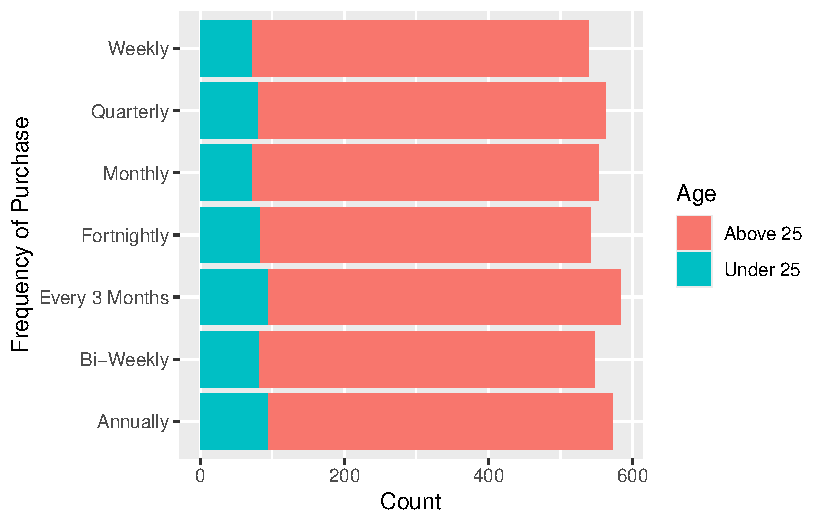
\includegraphics{Customer_Preference_Analytics_files/figure-pdf/unnamed-chunk-22-1.pdf}

}

\caption{Plots showing the frequency purchase in different age group}

\end{figure}%

The plot shows that the proportions of people Above 25 is quite higher
than Under 25. Moreover, both groups have high preference for the
purchasing every 3 months. Additionally, People both under and above 25
have higher frequency of purchase annually. Whereas, rest of the
Frequency of purchase categories also have some proportion of customers.
From the plot it can be said that there are not much of a difference in
frequency of purchase within groups.

\begin{verbatim}

    Pearson's Chi-squared test

data:  table(df_2$Age.bin, df_2$Frequency.of.Purchases)
X-squared = 4.8901, df = 6, p-value = 0.558
\end{verbatim}

The Chi-square test of Independence were not significant,
\(X^{2}(6, 3900) = 4.8901, p > 0.05\), this suggests that the Frequency
of Purchase and Age groups are independent of each other and there is
not enough evidence to conclude that there is any relation between two
variables.

\begin{figure}[H]

{\centering 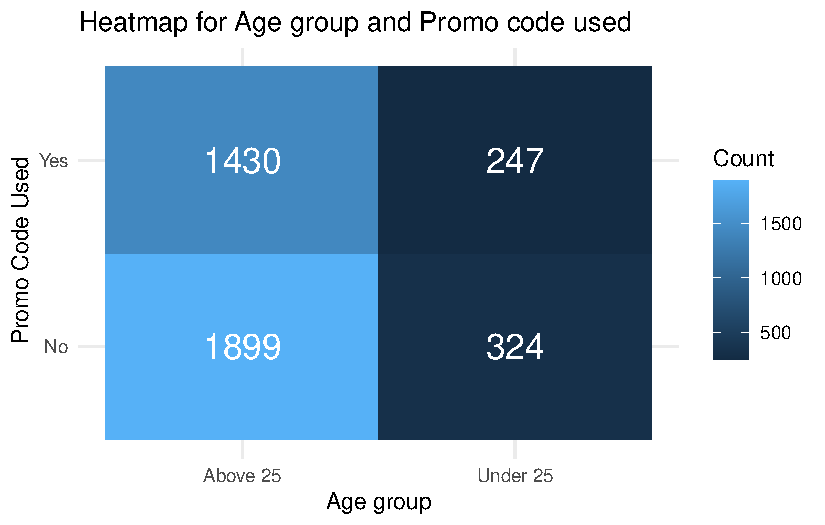
\includegraphics{Customer_Preference_Analytics_files/figure-pdf/unnamed-chunk-24-1.pdf}

}

\caption{Heatmap showing contingency table of Promo code used vs Age
Group}

\end{figure}%

The heatmap shows the contingency table between Age group and Promo Code
Used or not. Although there are less individual under 25 than above 25.
In addition, both the groups have higher number of individuals
\textbf{not using promo code} than those using promo code.

\begin{verbatim}

    Pearson's Chi-squared test with Yates' continuity correction

data:  age_promo_code
X-squared = 0.0078762, df = 1, p-value = 0.9293
\end{verbatim}

The pearson's chi-squared test shows that there is \textbf{no
relationship} between age groups and promo code use.

\begin{figure}[H]

{\centering 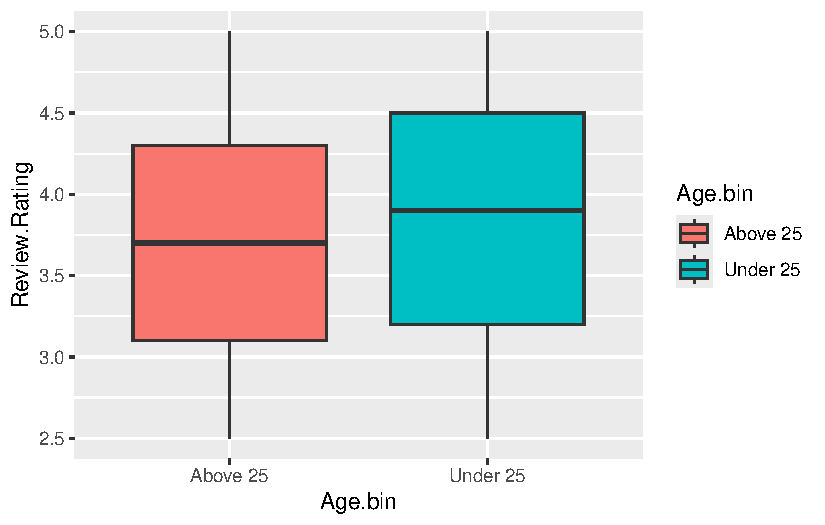
\includegraphics{Customer_Preference_Analytics_files/figure-pdf/unnamed-chunk-26-1.pdf}

}

\caption{Boxplot showing distributions of Review ratings in different
Age Groups}

\end{figure}%

The boxplots depicts that overall both the groups rate
\texttt{between\ 2.5\ and\ 5}. However, shoppers that are Above 25
having median rating below 3.75 while Under 25 usually rate higher with
median rating above 3.75. This hypothesis can be checked using a t-test
of independence.

Before conducting the test, assumption of t test needs to be checked

\begin{enumerate}
\def\labelenumi{\roman{enumi}.}
\tightlist
\item
  \textbf{Extreme Outliers}: Here, the continuous variable is checked to
  identify if there are any extreme outliers in the dataset.
\end{enumerate}

\begin{verbatim}
 [1] Age.bin                  Customer.ID              Age                     
 [4] Gender                   Item.Purchased           Category                
 [7] Purchase.Amount..USD.    Location                 Size                    
[10] Color                    Season                   Review.Rating           
[13] Subscription.Status      Payment.Method           Shipping.Type           
[16] Discount.Applied         Promo.Code.Used          Previous.Purchases      
[19] Preferred.Payment.Method Frequency.of.Purchases   is.outlier              
[22] is.extreme              
<0 rows> (or 0-length row.names)
\end{verbatim}

The output shows 0 rows which means there are no outliers or extreme
outliers in the Review rating variable.

\textbf{ii. Normality Test}: In this test the Shapiro-Wilks test is
conducted to check if there is normality in the distribution between
groups. Here if p-value is \textgreater{} than 0.05 than the data is
normally distributed.

\begin{verbatim}
# A tibble: 2 x 4
  Age.bin  variable      statistic        p
  <fct>    <chr>             <dbl>    <dbl>
1 Above 25 Review.Rating     0.957 2.02e-30
2 Under 25 Review.Rating     0.948 3.02e-13
\end{verbatim}

Unfortunately, the Shapiro-Wilks test failed to prove normality as
p-values are less than the significance level (0.05). A non-parametric
needs to be conducted.

\textbf{iii. Homogeneity Test}: In this assumption test, with the help
of the Levene's test, variance of different groups are checked if they
are homogeneous or heterogeneous.

\begin{verbatim}
# A tibble: 1 x 4
    df1   df2 statistic     p
  <int> <int>     <dbl> <dbl>
1     1  3898      1.15 0.283
\end{verbatim}

Levene's test proved the homogeneity in the variance of the two groups
as p-value(0.283) \textgreater{} 0.05.

\begin{verbatim}
# A tibble: 1 x 8
  .y.           group1   group2      n1    n2 statistic    df      p
* <chr>         <chr>    <chr>    <int> <int>     <dbl> <dbl>  <dbl>
1 Review.Rating Above 25 Under 25  3329   571     -2.37  773. 0.0178
\end{verbatim}

The results of the t-test suggest there is some relationship between
Review rating and Age groups, t(773) = -2.37, p \textless{} 0.05.

\begin{verbatim}
# A tibble: 1 x 7
  .y.           group1   group2   effsize    n1    n2 magnitude 
* <chr>         <chr>    <chr>      <dbl> <int> <int> <ord>     
1 Review.Rating Above 25 Under 25  -0.108  3329   571 negligible
\end{verbatim}

As per Cohen's D test, the relationship has a negligible effect between
Age and Review rating.

\begin{figure}[H]

{\centering 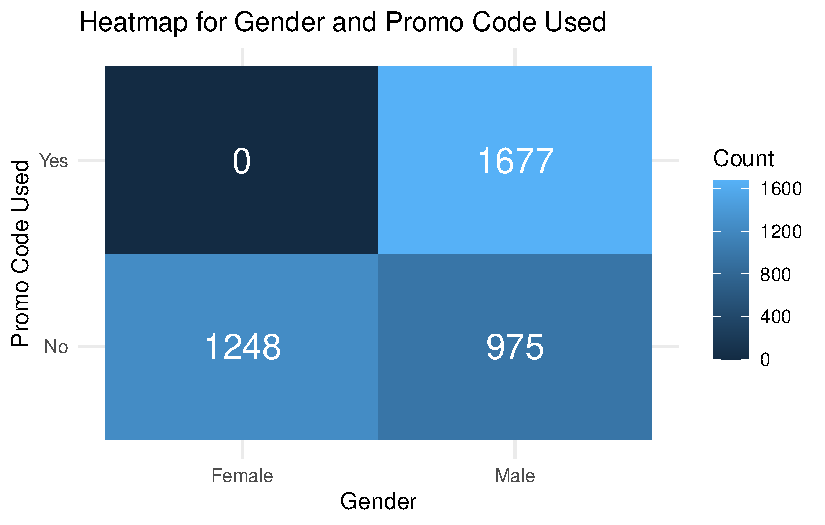
\includegraphics{Customer_Preference_Analytics_files/figure-pdf/unnamed-chunk-32-1.pdf}

}

\caption{Heatmap showing the contingency table between Gender and Promo
Code Use}

\end{figure}%

It is clear from the heat map that Females do not like to use Promo
codes whereas, on the other hand, Men highly use Promo codes.

\begin{verbatim}

    Pearson's Chi-squared test with Yates' continuity correction

data:  gender_promo_code
X-squared = 1381.9, df = 1, p-value < 2.2e-16
\end{verbatim}

\begin{verbatim}
  Dimension     Value        No       Yes
1    Female Residuals  37.20914 -37.20914
2    Female  p values   0.00000   0.00000
3      Male Residuals -37.20914  37.20914
4      Male  p values   0.00000   0.00000
\end{verbatim}

The results of the chi-square confirm that the p-value for Promo-code
use as \texttt{Yes} is less than 0.05 with residuals negative and males
having residuals having residuals in positive.

\begin{figure}[H]

{\centering 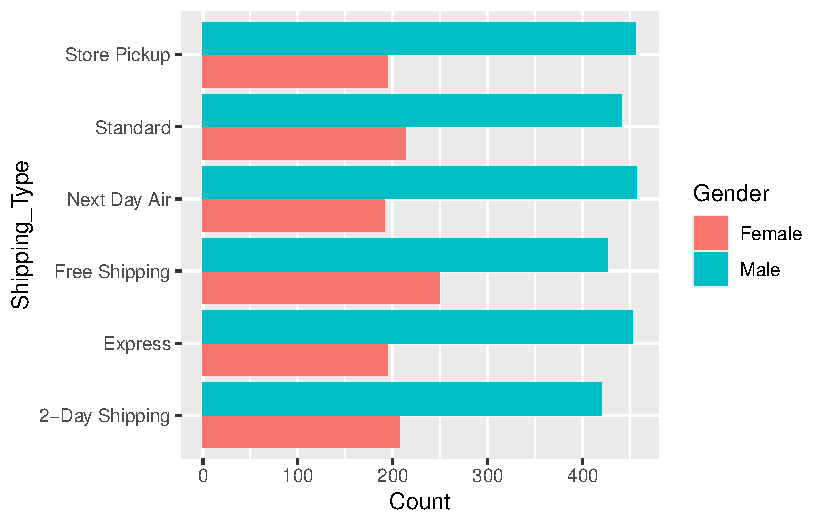
\includegraphics{Customer_Preference_Analytics_files/figure-pdf/unnamed-chunk-34-1.pdf}

}

\caption{Horizontal barchart showing}

\end{figure}%

The horizontally grouped bar chart depicts that Males have a higher
preference for Store Pickup, Next Day Air, and Express. Whereas Females
prefer Free Shipping highly.

\begin{verbatim}

    Pearson's Chi-squared test

data:  shipping_table
X-squared = 12.243, df = 5, p-value = 0.03161
\end{verbatim}

After conducting the chi-square test of independence between Gender and
Shipping type, it shows there is significance,
\(X^{2}(5,3900) = 12.243, p < 0.05\).

\begin{verbatim}
  Dimension     Value 2-Day Shipping   Express Free Shipping Next Day Air
1    Female Residuals       0.594365 -1.174532      2.994333    -1.508771
2    Female  p values       1.000000  1.000000      0.033006     1.000000
3      Male Residuals      -0.594365  1.174532     -2.994333     1.508771
4      Male  p values       1.000000  1.000000      0.033006     1.000000
    Standard Store Pickup
1  0.3418083    -1.289533
2  1.0000000     1.000000
3 -0.3418083     1.289533
4  1.0000000     1.000000
\end{verbatim}

From the post-hoc test, it is clear that only free shipping has a
p-value less than 0.05. Based on residuals Females have a higher
preference for free shipping than Males. Lastly, other types of shipping
methods do not have much significance with gender.

\newpage

\section{Bibiliography}\label{bibiliography}

\phantomsection\label{refs}
\begin{CSLReferences}{1}{0}
\bibitem[\citeproctext]{ref-kaggle_customer_shopping}
bhadramohit. 2024. {``Customer Shopping Latest Trends Dataset.''}
\url{https://www.kaggle.com/datasets/bhadramohit/customer-shopping-latest-trends-dataset}.

\bibitem[\citeproctext]{ref-cleofasbrand}
Cleofas, Maria Arielle, Yogi Tri Prasetyo, Ardvin Kester S Ong, and
Satria Fadil Persada. n.d. {``Brand or Clothing Function? Consumer
Preference Analysis on Clothing Apparel Attributes and Design: A
Conjoint Analysis Approach.''}

\bibitem[\citeproctext]{ref-delimarta2021customer}
Delimarta, Florencia Devina, and Raden Aswin Rahadi. 2021. {``Customer
Preferences on Sustainable Fashion Purchases: A Conceptual Model.''}
\emph{International Journal of Entrepreneurship and Management
Practices} 4 (13): 78--88.

\bibitem[\citeproctext]{ref-giri2019customer}
Giri, Chandadevi, Sebastien Thomassey, and Xianyi Zeng. 2019.
{``Customer Analytics in Fashion Retail Industry.''} In \emph{Functional
Textiles and Clothing}, 349--61. Springer.

\bibitem[\citeproctext]{ref-glinska2017customer}
Glińska, Ewa, and Ewelina Tomaszewska. 2017. {``Customer Preferences
Related to Shopping Online.''} \emph{Annales Universitatis Mariae
Curie-Sk{ł}odowska, Sectio H--Oeconomia} 51 (2): 87.

\bibitem[\citeproctext]{ref-kod1customer}
Kod, JEL. n.d. {``Customer Preferences Related to Shopping Online.''}
\emph{Chemistry} 1: 56.

\bibitem[\citeproctext]{ref-okofu2024pilot}
Okofu, Sebastina Nkechi, Kizito Eluemunor Anazia, Maureen Ifeanyi
Akazue, Margaret Dumebi Okpor, Amanda Enadona Oweimieto, Clive Ebomagune
Asuai, Geoffrey Augustine Nwokolo, Arnold Adimabua Ojugo, and Emmanuel
Obiajulu Ojei. 2024. {``Pilot Study on Consumer Preference, Intentions
and Trust on Purchasing-Pattern for Online Virtual Shops.''} \emph{Int.
J. Adv. Comput. Sci. Appl} 15 (7): 804--11.

\bibitem[\citeproctext]{ref-statista2023global}
Statista. 2023. {``Global Online Fashion Market Value from 2017 to
2027.''}
\url{https://www.statista.com/statistics/228706/global-online-fashion-market-value/}.

\bibitem[\citeproctext]{ref-sulianta2024revealing}
Sulianta, Feri, Khaerani Ulfah, and Endang Amalia. 2024. {``Revealing
Consumer Preferences in the Fashion Industry Using k-Means
Clustering.''} \emph{International Journal of Engineering Continuity} 3
(2): 34--53.

\bibitem[\citeproctext]{ref-suzianti2015customer}
Suzianti, Amalia, Nurza Dwi Prisca Faradilla, and Shabila Anjani. 2015.
{``Customer Preference Analysis on Fashion Online Shops Using the Kano
Model and Conjoint Analysis.''} \emph{International Journal of
Technology} 6 (5): 881--85.

\bibitem[\citeproctext]{ref-wibowo2024exploring}
Wibowo, Amira Luthfiyya. 2024. {``Exploring Santoon's Customers'
Preferences That Affect Their Purchase Decision for Buying Fashion
Products.''} \emph{Journal of Consumer Studies and Applied Marketing} 2
(2): 139--45.

\end{CSLReferences}




\end{document}
